\documentclass[10pt]{article}
\usepackage[spanish]{babel}
\usepackage[utf8]{inputenc}
\usepackage{graphicx}
\usepackage{amsmath,amsthm,amssymb}
\usepackage{amsfonts}
\usepackage{bbold}
\usepackage[margin=1in]{geometry}
\usepackage[export]{adjustbox}
\usepackage{grffile}
\usepackage{titling}
\usepackage{titlesec}
\usepackage{mdwlist}
\usepackage{float}
\usepackage{fancyhdr}
\usepackage{hyperref}
\usepackage{mathtools}
\usepackage[sort&compress]{natbib}
\usepackage[ruled,vlined]{algorithm2e}
\usepackage{multirow}

\selectlanguage{spanish}

% \pagecolor{black}
% \color{white}

\DeclareTextCommandDefault{\textregistered}{\textcircled{ \check@mathfonts\fontsize\sf@size\z@\math@fontsfalse\selectfont R}}

\newcommand{\mybreak}{%
  \par
  \nointerlineskip
  \cleaders\vbox to 5ex{%
    \vss
    \hbox to \textwidth{\hss\vrule width 1\textwidth height 0.2pt depth 0.2pt\hss}
    \vss
  }\vskip5ex
}

\renewcommand{\headrulewidth}{0pt}

\renewcommand\maketitlehooka{
\vspace{-2cm}
\noindent
\begin{minipage}{0.1\textwidth}

\includegraphics[width=\linewidth]{Logo.png}
\end{minipage}
\begin{minipage}{0.8\textwidth}\raggedright
\ \textbf{Facultad de Ingeniería}\\
\ \textbf{Mastering ML: Tiny and Simple - Laboratorio Edge Impulse}\\
\ PROFESOR: Elkin Garcia
\end{minipage}
\mybreak
}

\begin{document}
\title{Tarea 1}
\date{}
\author{}
\maketitle
\vspace{-17ex}
\begin{table}[h]
\begin{center}
	\begin{tabular}{c c c c}
		\textbf{Apellidos} & \textbf{Nombres} & \textbf{Código} & \textbf{Login}\\
		\hline
		Mantilla Redondo & Alejandro & 201711304 & a.mantillar \\
		Patiño & Cristhian & NA & NA\\
		\hline
	\end{tabular}
\end{center}
\label{tab:Nombres}
\end{table}

\section*{Equipo}

Somos Cristhian y Alejandro, un equipo de investigadores en \textit{Machine Learning} dedicado al desarrollo de modelos predictivos de punta y a su despliegue en soluciones tecnológicas tipo \textit{edge computing} y en sistemas embebidos.

\section*{Datos}

Identificamos en un inicio que técnicas de reducción de dimensionalidad sencillas como PCA o t-SNE son suficiente para agrupar de manera evidente los audios que pertenecen a una misma categoría. Las figuras \ref{fig:PCA} y \ref{fig:tsne} nos muestran que un modelo de \textit{machine learning} puede ser apropiado para predecir de manera acertada la categoría de los audios.

\begin{figure}
    \centering
    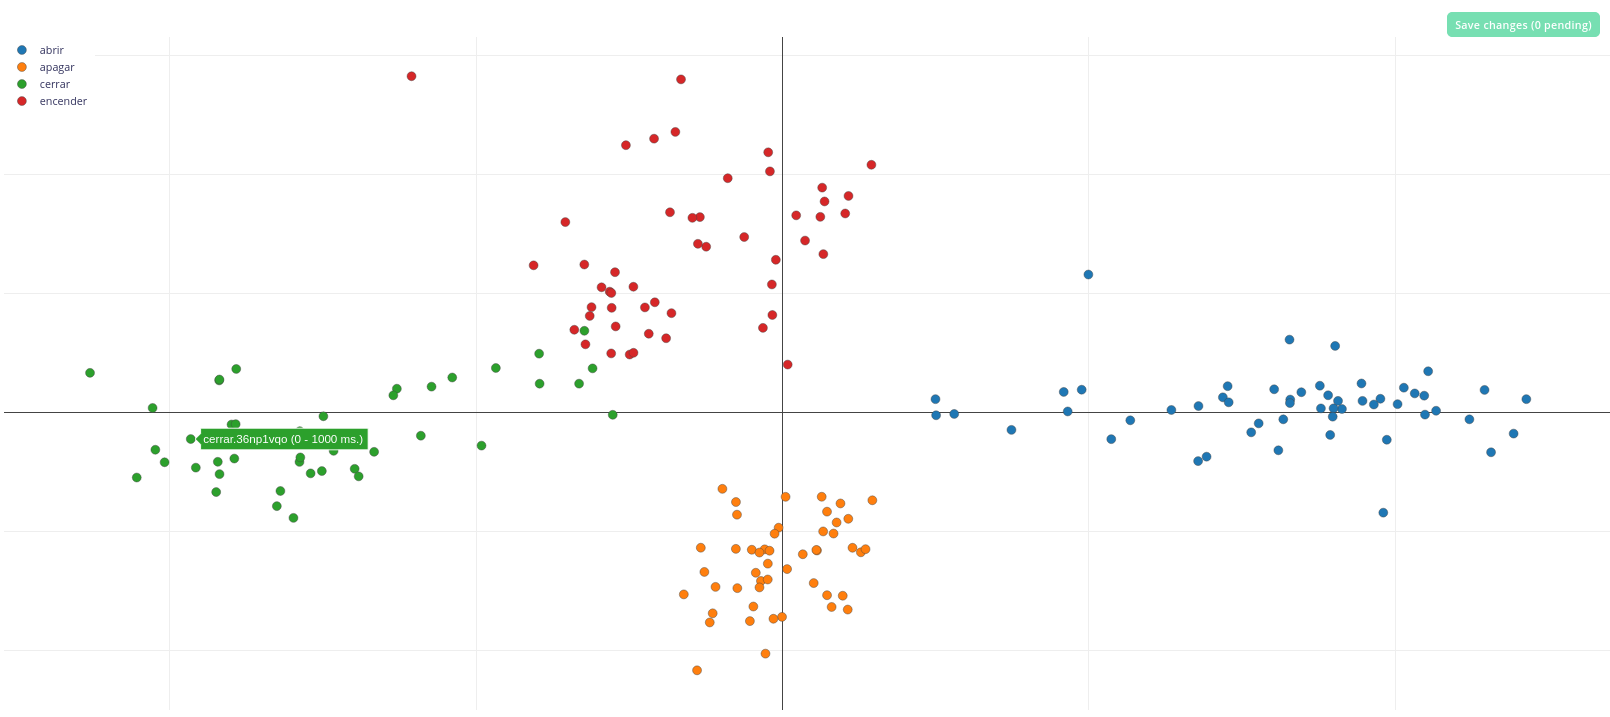
\includegraphics[width=0.75\textwidth]{PCA Data explorer.png}
    \caption{Descomposición PCA.}
    \label{fig:PCA}
\end{figure}

\begin{figure}
    \centering
    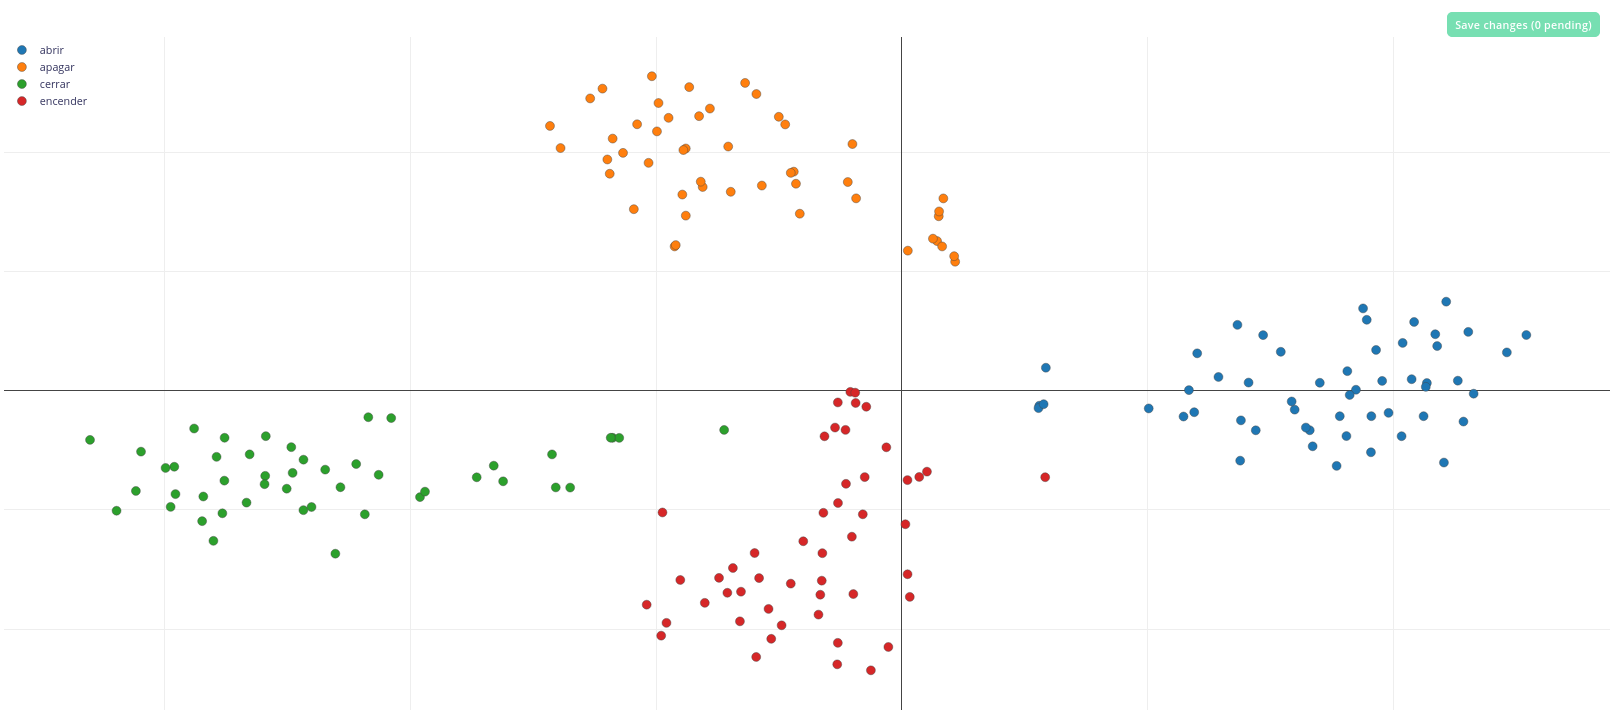
\includegraphics[width=0.75\textwidth]{t-sne - Data Explorer.png}
    \caption{Descomposición t-SNE.}
    \label{fig:tsne}
\end{figure}



\section*{Desarrollo}

Exploraremos las distintas arquitecturas exploradas para el \textit{pipeline} que dedicamos a la predicción de audios, según la palabra que corresponda. Expondremos los beneficios y desventajas de cada arquitectura y los resultados respectivos. 

\subsection*{Arquitecturas}

\subsubsection*{Syntiant - \textit{DNN} (Keras)}

Este flujo de trabajo toma el \textit{dataset} de entrenamiento y lo codifica según un bloque de preprocesamiento tipo Syntiant. La documentación de Edge Impulse indica que calcula características de energía tipo \textit{log Mel-filterbank}. La intención es caracterizar los audios según su descomposición espectral.

El modelo de redes neuronales profunda escogido tiene la configuración de la figura \ref{fig:config1}. Nótese que el proceso de entrenamiento considera 200 épocas, un learning rate inicial de 0.0005 (variable porque el optimizador es Adam), y un preprocesamiento de \textit{data augmentation}. Se considera un \textit{dataset} de validación pero excluimos el desempeño a lo largo de las épocas de nnuestro análisis.

\begin{figure}
    \centering
    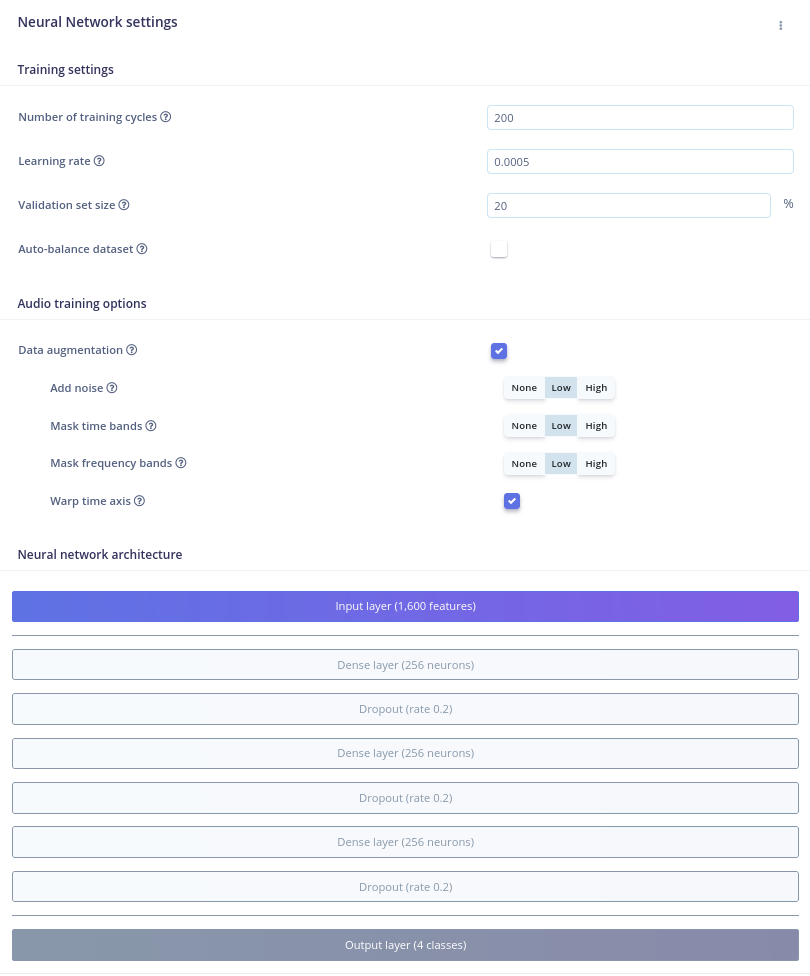
\includegraphics[width=0.75\textwidth]{Syntiant to DNN Config.png}
    \caption{Keras DNN configuración 1.}
    \label{fig:config1}
\end{figure}

\subsubsection*{Syntiant - \textit{DNN} (Keras)}

Sobre el mismo flujo de trabajo anterior consideramos el modelo con solo 100 épocas y menos características de \textit{data augmentation}, es decir, sin la opción de \textit{Warp time axis}. La configuración de esta red pueden verla en la figura \ref{fig:config2}.

\begin{figure}
    \centering
    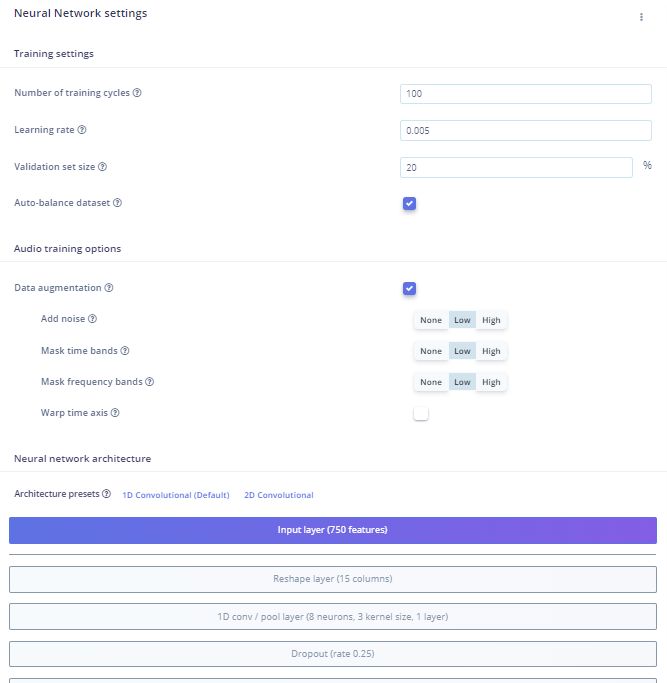
\includegraphics[width=0.75\textwidth]{Syntiant to DNN Config 2.png}
    \caption{Keras DNN configuración 2.}
    \label{fig:config2}
\end{figure}

\subsubsection*{MFCC - \textit{DNN} (Keras)}

Ahora con una arquitectura distinta (particularmente por la cantidad de nodos en la capa de entrada), consideramos un preprocesamiento tipo MFCC. La intención es generar características estructuradas tipo \textit{Mel Frequency Cepstral Coefficients}. Los hiperparámetros del modelo \textit{DNN} son iguales al anterior pero el proceso de entrenamiento no contempla data augmentation, por lo que podríamos sospechar que el resultado sería menos robusto, su poniendo que los datos transformados por este proceso son razonables y representativos del sistema. Encuentre la configuración en la figura \ref{fig:config3}.

\begin{figure}
    \centering
    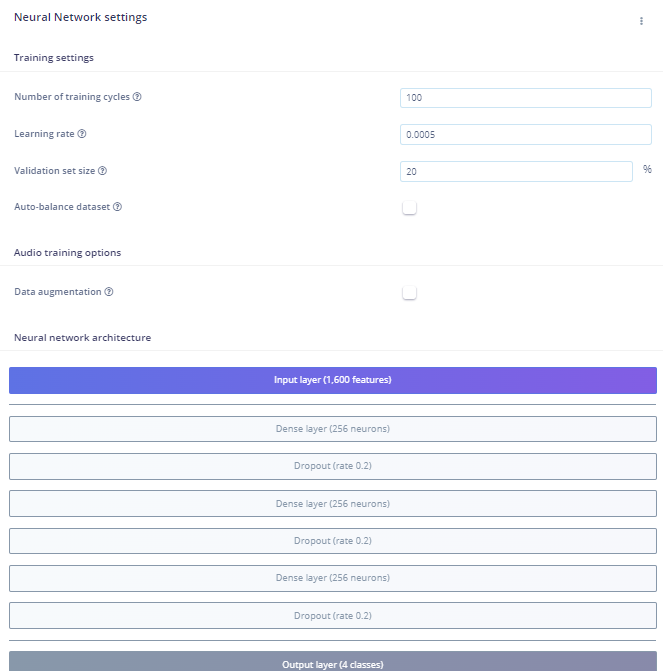
\includegraphics[width=0.75\textwidth]{MFCC to DNN Config.png}
    \caption{Keras DNN configuración 3.}
    \label{fig:config3}
\end{figure}

\subsection*{Desempeño}

Enfocamos nuestro análisis en los datos de prueba para validar el desempeño real de nuestros modelos. En general, todos los modelos son altamente capaces y efectivos.

\subsubsection*{Syntiant - \textit{DNN} (Keras)}

Identificamos en la figura \ref{fig:desempeno1} que, para el \textit{dataset} de prueba, solo se predijo de manera errada un audio de la palabra \"abrir\".

\begin{figure}
    \centering
    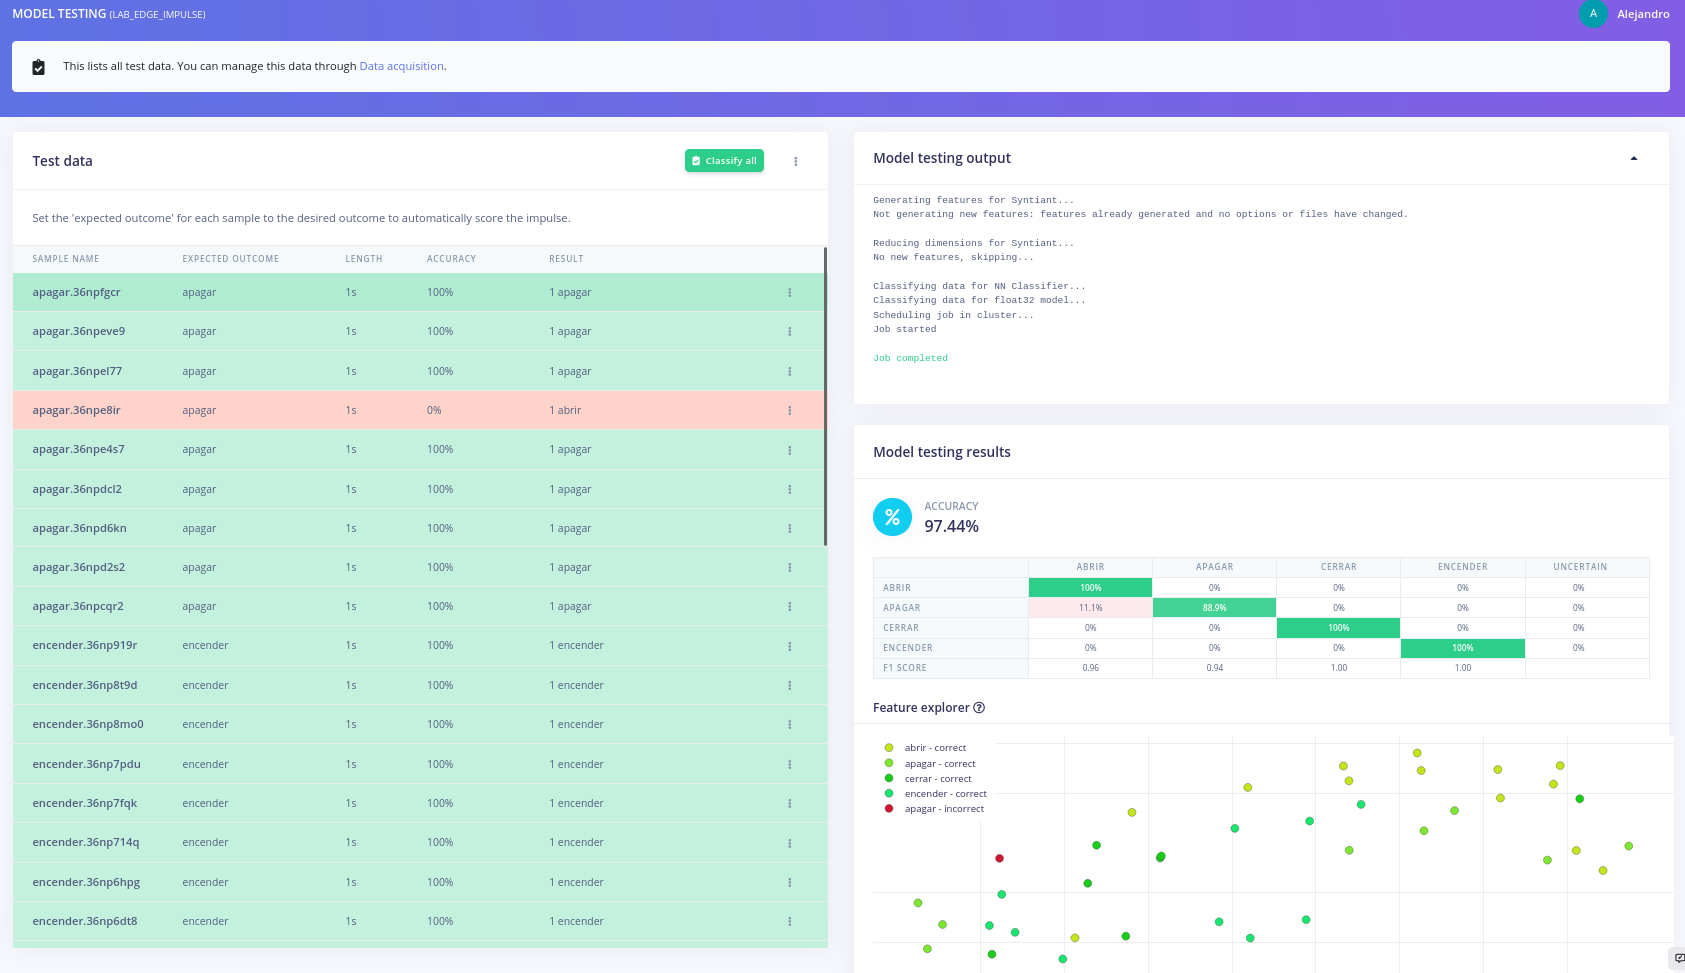
\includegraphics[width=0.75\textwidth]{End classification - Syntiant to DNN.png}
    \caption{Desempeño 1.}
    \label{fig:desempeno1}
\end{figure}

\subsubsection*{Syntiant - \textit{DNN} (Keras)}

Identificamos en la figura \ref{fig:desempeno2} que, para el \textit{dataset} de prueba, se predijo de manera acertada el 100\% de los datos de prueba.

\begin{figure}
    \centering
    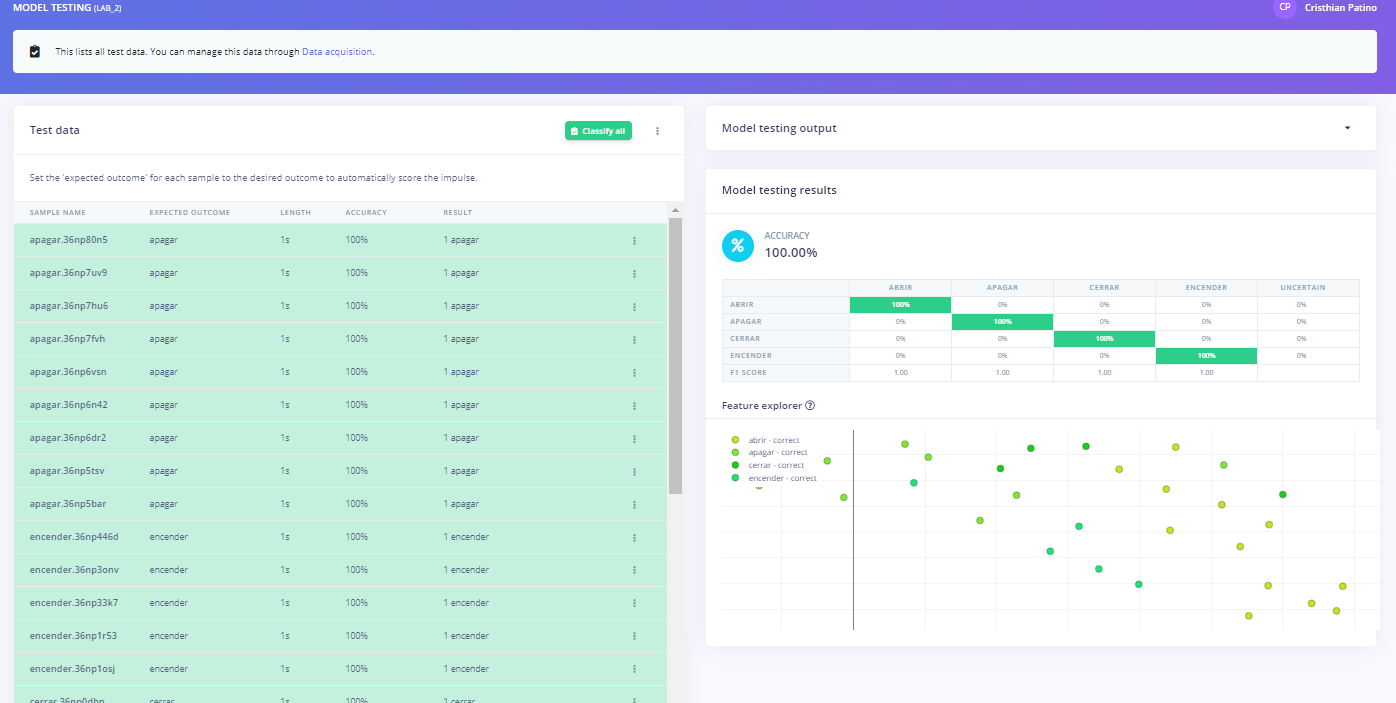
\includegraphics[width=0.75\textwidth]{End classification - Syntiant to DNN 2.png}
    \caption{Desempeño 2.}
    \label{fig:desempeno2}
\end{figure}

\subsubsection*{MFCC - \textit{DNN} (Keras)}

Identificamos en la figura \ref{fig:desempeno3} que, para el \textit{dataset} de prueba, hubo errores en la predicción de audios de las palabras \"encender\", \"abrir\" y \"apagar\". Particularmente, las palabras \"abrir\" y \"encender\" fueron confundidas con otras dos palabras en más de una ocasión.

\begin{figure}
    \centering
    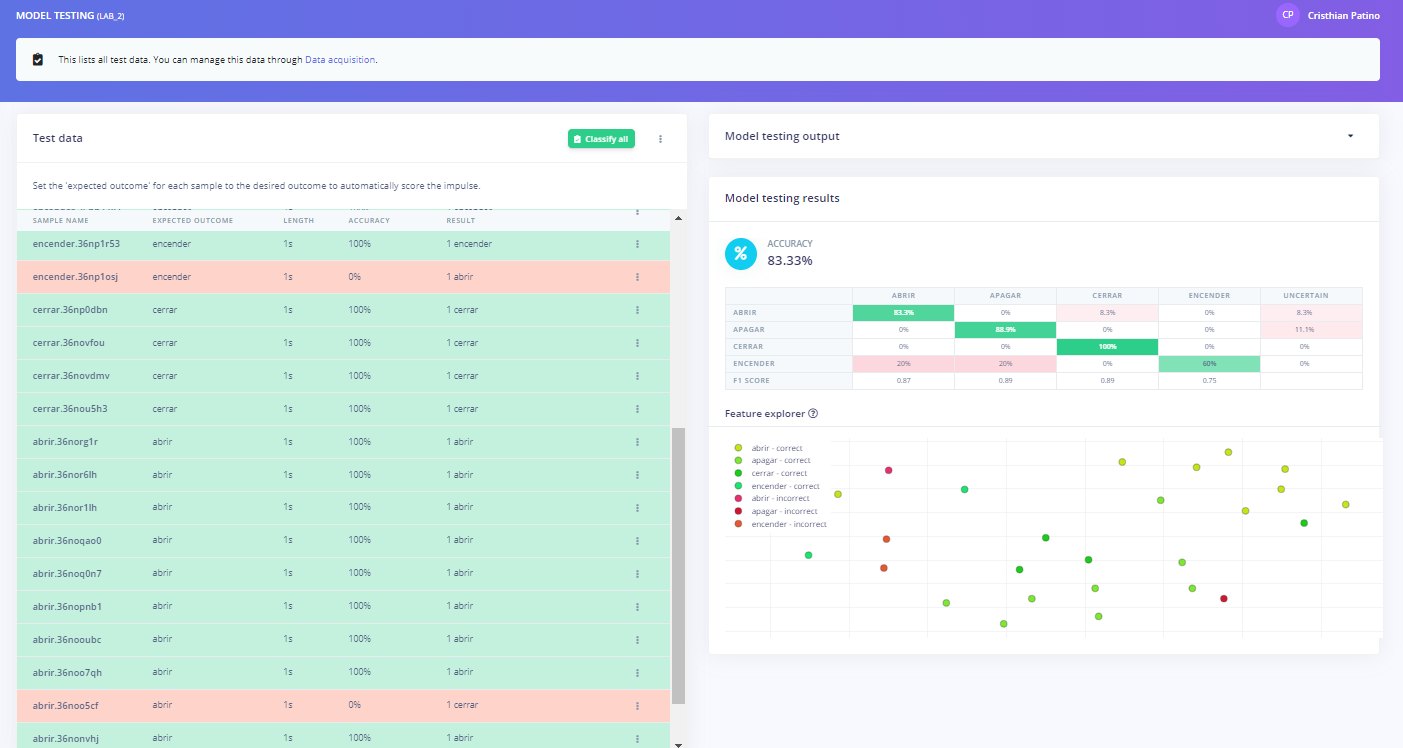
\includegraphics[width=0.75\textwidth]{End classification - MFCC to DNN.png}
    \caption{Desempeño 3.}
    \label{fig:desempeno3}
\end{figure}

El resultado definitivo es que el mejor modelo es la segunda versión de Syntiant con un \textit{DNN}, pece a nuestras predicciones de que las limitaciones en el proceso de aprendizaje resultarían en un peor modelo.

Para mejorar el desempeño de los modelos, aunque de por sí son altamente efectivos, recomendamos probar redes neuronales más especializadas, como las tipo RNN, que aprovechen la correlación secuencial de los audios. También, tener datos más diversos, registrados con distintas voces y con más fluctiaciones puede ayudar a introducir variabilidad en los datos y que los modelos puedan detectar de manera acertada la clase de audios poco similares al resto de los datos.



%Bibliografía
%\clearpage 
%\bibliographystyle{plain}
%\bibliography{Biblio}
%Fin bibliografía

\end{document}